\chapter{Algorithms} \label{algo}
For the task of density estimation, we investigated several Markov chain methods to sample from the posterior distribution of a DPM model. \\
Starting from the hierarchical model (\ref{dpm-1}), a first direct approach is simply drawing values for each $\boldsymbol\theta_i$ from its conditional distribution, given the data and the other $\boldsymbol\theta_j$.
However, as previously discussed, we have high probability for ties among them which can lead to slow convergence, since the $\boldsymbol\theta_i$ are not updated for more than one observation simultaneously. \\
For this reason, special attention was paid to the three methods we present in this chapter.
These are all \emph{Gibbs sampler} methods, that is, each value is updated by drawing from its own conditional distribution given all other values.
Moreover, these three methods have a common base structure, sharing the two steps for the sampling of the allocations $\mathbf{c}$ and of the unique values $\boldsymbol\phi_c$.
The set of allocations and unique values at a given iteration constitutes the \emph{state} of that iteration.
As the state is being updated at each iteration, a \emph{chain} is formed and the mean of the state values eventually reaches convergence, as well as the estimate for the data distribution, as we will see in section \ref{dens-estim}.
Moreover, all methods can be extended with additional steps for hierarchical extensions.
For example, we can place priors to hyperparameters of the centering measure $G_0$ or to the total mass $M$.

\section{Neal's Algorithm 2} \label{neal2}
In order to speed up convergence in case of ties, Neal first proposed (see \cite{neal} section 3 as well as \cite{book} chapter 2) a more efficient Gibbs sampling method based on the discrete model (\ref{dpm-disc}), but where the mixing proportions $\textbf{p}$ have been integrated out.
We will refer to this method as Neal's Algorithm 2, or \verb|Neal2| for short.
Before getting to the algorithm, let us start from the discrete model (\ref{dpm-disc}).
Assuming that the current state of Markov chain is composed of $(c_1,\dots,c_n)$  and the unique values $\boldsymbol\phi_c$ for all $c=1,\dots,k$, the Gibbs sampler should first draw a new value $c$ for each $c_i$ according to the following probabilities:
\begin{align}
	\hspace{-25pt}
	\vspace{-12pt}
	\text{If $c=c_j$ for some $j$: }
	\PP(c_{i}=c | \boldsymbol c_{-i}, y_{i},\boldsymbol{\phi}_1,\dots,\boldsymbol{\phi}_k) \propto \frac{n_{-i,c} + M/{K}}{n-1+M} f(y_{i}|\boldsymbol\phi_{c}) 
\end{align}
where $\boldsymbol c_{-i}$ is $\boldsymbol c$ minus the $i$-th component, and $n_{-i,c}$ is the number of $c_j$ equal to $c$ excluding $c_i$.
The transition to the infinite case, that is, to the reference DPM model (\ref{dpm-2}), is handled by taking the limit as $K$ goes to infinity in the conditional distribution of $c_i$, which becomes as follows:
\begin{equation}
	\begin{aligned} \label{probasneal2}
	\hspace{-25pt}
	\vspace{-12pt}
	\text{If $c=c_j$ for some $j$: }
	\PP(c_{i}=c | \boldsymbol c_{-i}, y_{i}, \boldsymbol{\phi}_1,\dots,\boldsymbol{\phi}_k) &\propto \frac{n_{-i,c} }{n-1+M} f(y_{i}|\boldsymbol\phi_{c}) \\
	\PP(c_{i}\neq c_{j} \text{ for all } j | \boldsymbol c_{-i}, y_{i}, \boldsymbol{\phi}_1,\dots,\boldsymbol{\phi}_k) &\propto \frac{M }{n-1+M} \int_{\Theta} f(y_{i}|\boldsymbol\theta) \, G_0(\de\boldsymbol\theta)
	\end{aligned}
\end{equation}
and considering only the $\boldsymbol\phi_c$ associated with some observation, keeping the sampling finite and thus computationally feasible.
The former expression is proportional to the cardinality of that cluster (excluding the $i$-th observation), while the latter is instead proportional to the total mass $M$ and represents the probability of creating a new cluster.
This is exactly the Polya's urn scheme we touched upon earlier.
Moreover, the integral $m(y_i) = \int_{\Theta} f(y_{i}|\boldsymbol\theta) \, G_0(\de\boldsymbol\theta)$ represents the \emph{marginal distribution} of the data points evaluated in $y_i$. \\
Let us now introduce the actual \verb|Neal2| algorithm, which works iteratively in two steps, in which we sample $(\boldsymbol{c}_1,\dots,\boldsymbol{c}_n)$ and $(\boldsymbol{\phi}_1,\dots,\boldsymbol{\phi}_k)$, respectively.
First, for each observation $i$, $c_i$ is updated according to the conditional probabilities (\ref{probasneal2}).
It can be set either to one of the other components currently associated with some observation, or to a new mixture component.
If the new value of $c_i$ is different from all the other $c_j$, a value for $\boldsymbol\phi_{c_i}$ is created by drawing it from the posterior distribution $H_i$, given the prior $G_0$ and the single observation $y_i$; this means that in this case, a new cluster has been created. \\
Then, for all clusters, the sampling of their unique value $\boldsymbol\phi_c$ is conducted by considering their posterior distribution given the prior $G_0$ and all observations belonging to that cluster.
The probability of setting $c_i$ to a new component involves the computation of the marginal, which is difficult to compute in the non-conjugate case, as well as the sampling from the posterior $H_i$.
For this reason, the algorithm is only used under conjugacy and hence it is possible to exactly compute the integral.

\section{Neal's Algorithm 8} \label{neal8}
To handle non-conjugate priors, Neal proposed (see \cite{neal} section 6 and \cite{book} chapter 2) a second Markov chain sampling procedure, the \verb|Neal8| algorithm, where the state is extended by the addition of $m$ auxiliary parameters.
This technique allows to update the $c_i$ while avoiding the integration with respect to $G_0$ for the computation of the marginal. \\
In this case the sampling probabilities for the $c_i$ given all other $c_j$ are:
\begin{equation}
	\begin{aligned}
		\hspace{-25pt}
		\vspace{-12pt}
		\text{If $c=c_j$ for some $j$: } \PP(c_i=c | \boldsymbol c_{-i}) &= \frac{n_{-i,c}}{n-1+M}   \\
		\PP(c_{i}\neq c_{j} \text{ for all } j) &=\frac{M }{n-1+M}
	\end{aligned}	
\end{equation}
where the latter probability of creating a new cluster is evenly split among the $m$ auxiliary components, which will also be referred to as the \emph{auxiliary blocks}.
Maintaining the same structure as the \verb|Neal2| algorithm, \verb|Neal8| is composed of two steps, where the components of the Markov chain state $(\boldsymbol{c}_1,\dots,\boldsymbol{c}_n)$ and $(\boldsymbol{\phi}_1,\dots,\boldsymbol{\phi}_k)$ are repeatedly sampled.
\begin{figure}[h]
    \centering
    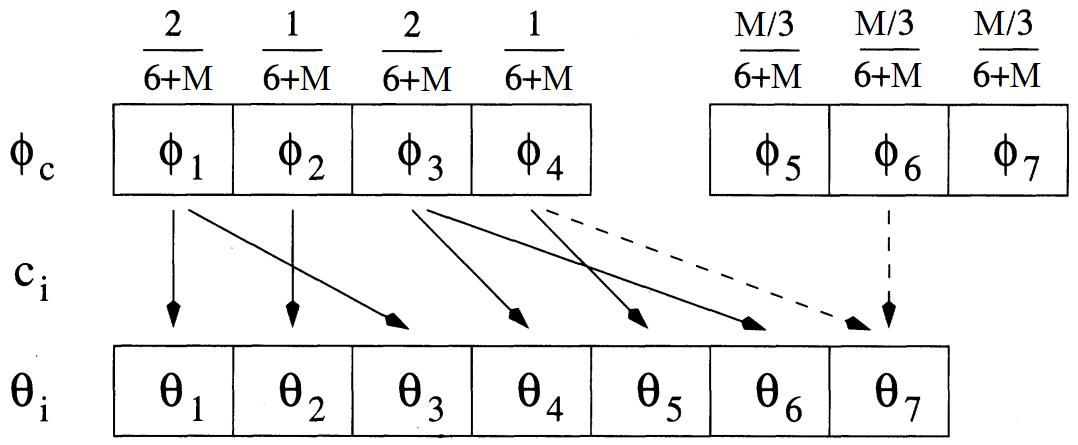
\includegraphics[width=0.9\textwidth]{etc/neal8.png}
    \captionsetup{labelformat=empty}
    \caption{Graphical representation of the variables: the allocations are visualized as arrows linking each $\boldsymbol\theta_i$ with either one of the four old clusters or one of the new components (image taken from \cite{neal})}
    \label{fig:neal8}
\end{figure}

The first step scans all the observations and evaluates each $c_i$.
If it is equal to some other $c_j$, i.e. if the current cluster of observation $i$ is not a singleton, then all auxiliary variables are iid drawn from $G_0$.
If instead the cluster corresponding to $c_i$ is a singleton, then it is linked to one of the auxiliary blocks (i.e. the first one, without loss of generality) while keeping its old unique value $\boldsymbol\phi_{c_i}$ (as shown in the above figure), whereas the other blocks are drawn normally from $G_0$ as before.
Then, $c_i$ is updated according to the following conditional probabilities:
\begin{equation}
	\begin{aligned} \label{neal8prob}
		\PP(c_{i}=c | \boldsymbol c_{-i}, y_{i}, \boldsymbol\phi_{1},\dots,\boldsymbol\phi_{h}) \propto
		\begin{cases}
			\dfrac{n_{-i,c}}{n-1+M}f(y_{i}|\boldsymbol\phi_{c}), & \mbox{for } 1 \leq c \leq k^{-} \\
			\\
			\dfrac{M/m}{n-1+M}f(y_{i}|\boldsymbol\phi_{c}), & \mbox{for } k^{-}+1 < c \leq h,
		\end{cases}
	\end{aligned}
\end{equation}
indicating with $k^{-}$ the number of distinct $c_j$ excluding the current $c_i$ and setting $h=k^{-}+m$.
Again, the probabilities of being placed in an already existing cluster or in a newly created cluster are proportional to the cluster's cardinality (sans observation $i$) and to the total mass, respectively. \\
Once all the $\boldsymbol\phi_c$ that are no longer associated with any observation are discarded, the algorithm proceeds, for each cluster, with the sampling of $\boldsymbol\phi_c$ from the posterior computed with the observations of the specific cluster, similarly to the \verb|Neal2| algorithm.

\section{Blocked Gibbs}
Another Gibbs sampling method that is applicable in the considered DPM model is the one proposed by Ishwaran and James (see \cite{james} section 5), where the prior $P$ is assumed to be a finite dimensional stick-breaking measure, allowing the update of whole blocks of parameters.
A key point of the method is that it does not marginalize over the prior; instead, by grouping more variables together, it samples from their joint distribution conditioned on all other variables.
This sampler needs to draw from the following conditionals:
\begin{align}
	\boldsymbol\phi_1,\dots,\boldsymbol\phi_k &\sim \Lc(\cdot | c_1,\dots,c_n, \boldsymbol{y}) \nonumber \\
	c_1,\dots,c_n &\sim \Lc (\cdot | \boldsymbol\phi_1,\dots,\boldsymbol\phi_k,\boldsymbol{p}, \boldsymbol{y}) \nonumber \\
	\boldsymbol{p} &\sim \Lc (\cdot | c_1,\dots,c_n) \nonumber
\end{align}
The drawing of the unique values can also be handled in the non-conjugate case by applying standard Markov chain Monte Carlo methods. \\
This algorithm is not explored in detail as it has not implemented yet in our library.
For a full explanation, see \cite{james}.
